\documentclass[12pt,a4paper,oneside]{report}

% --- Packages ---
\usepackage[utf8]{inputenc}
\usepackage[T1]{fontenc}
\usepackage[margin=1in]{geometry}
\usepackage{graphicx}
\usepackage{amsmath,amssymb}
\usepackage{booktabs}
\usepackage{tabularx}
\usepackage{xcolor}
\usepackage{listings}
\usepackage{hyperref}
\usepackage{fancyhdr}
\usepackage{titlesec}
\usepackage{microtype}
\usepackage{setspace}

\onehalfspacing

% --- Colors ---
\definecolor{primaryblue}{RGB}{26,115,232}
\definecolor{vcedark}{RGB}{20,40,80}
\definecolor{codebg}{RGB}{245,247,250}
\definecolor{codegray}{RGB}{100,100,100}

% --- Hyperref Setup ---
\hypersetup{
    colorlinks=true,
    linkcolor=vcedark,
    citecolor=primaryblue,
    urlcolor=primaryblue
}

% --- Listings Setup ---
\lstset{
    backgroundcolor=\color{codebg},
    basicstyle=\ttfamily\footnotesize,
    breaklines=true,
    frame=single,
    rulecolor=\color{black!20},
    keywordstyle=\color{primaryblue}\bfseries,
    commentstyle=\color{codegray}\itshape,
    stringstyle=\color{teal},
    tabsize=2,
    showstringspaces=false
}

% --- Header and Footer ---
\pagestyle{fancy}
\fancyhf{}
\fancyhead[L]{\small\nouppercase{\leftmark}}
\fancyhead[R]{\small\thepage}
\renewcommand{\headrulewidth}{0.5pt}

\fancypagestyle{plain}{
    \fancyhf{}
    \fancyfoot[C]{\thepage}
    \renewcommand{\headrulewidth}{0pt}
}

\begin{document}

% =============================================================================
% COVER PAGE
% =============================================================================
\begin{titlepage}
\begin{center}
    {\Large\bfseries\color{vcedark} VASAVI COLLEGE OF ENGINEERING (AUTONOMOUS)}\\[0.2cm]
    {\small (Affiliated to Osmania University, Approved by AICTE, Accredited by NAAC with A++ Grade)}\\[0.2cm]
    {\small Ibrahimbagh, Hyderabad -- 500031, Telangana, India}\\[1.0cm]

    
\includegraphics[width=0.25\textwidth]{figures/vce_logo.png}\\[1.0cm]

    {\large\bfseries A COURSE BASED PROJECT REPORT}\\[0.2cm]
    {\normalsize\itshape submitted in partial fulfillment of the requirements for the award of}\\[0.2cm]
    {\normalsize\bfseries HONOURS DEGREE IN SYSTEM ON CHIP DESIGN}\\[0.2cm]
    {\normalsize in}\\[0.2cm]
    {\normalsize\bfseries ELECTRONICS AND COMMUNICATION ENGINEERING}\\[1.0cm]

    {\large\bfseries\color{vcedark} RISC-V VeeR EL2 BASED SENSOR MONITORING AND SIGNAL PROCESSING SoC}\\[1.2cm]

    \begin{minipage}{0.45\textwidth}
        \textbf{Submitted by:}\\[0.1cm]
        \textbf{Veeramalla Akshay}\\
        Roll No: 1602-23-735-130\\
        Department of ECE
    \end{minipage}
    \hfill
    \begin{minipage}{0.45\textwidth}
        \raggedleft
        \textbf{Under the Guidance of:}\\[0.1cm]
        \textbf{Dr. M. Praveen Kumar}\\
        Assistant Professor\\
        Department of ECE
    \end{minipage}

    \vfill
    {\bfseries ACADEMIC YEAR 2026 -- 2027}
\end{center}
\end{titlepage}

% =============================================================================
% FRONT MATTER
% =============================================================================
\pagenumbering{roman}
\setcounter{page}{2}

\chapter*{Certificate of Original Work}
\addcontentsline{toc}{chapter}{Certificate}
This is to certify that the project report entitled \textbf{``RISC-V VeeR EL2 BASED SENSOR MONITORING AND SIGNAL PROCESSING SoC''} is a bonafide record of course based project work carried out by \textbf{Veeramalla Akshay} (Roll No: \texttt{1602-23-735-130}), under my guidance and supervision in the Department of Electronics and Communication Engineering, Vasavi College of Engineering (Autonomous), Hyderabad, in partial fulfillment of the requirements for the award of the Honours Degree in System on Chip Design during the academic year 2026 -- 2027.

\vspace{3cm}
\noindent
\begin{minipage}{0.45\textwidth}
    \textbf{Dr. M. Praveen Kumar}\\
    Internal Supervisor\\
    Assistant Professor, Dept. of ECE
\end{minipage}
\hfill
\begin{minipage}{0.45\textwidth}
    \raggedleft
    \textbf{Dr. E. Sreenivasa Rao}\\
    Professor \& Head of Department\\
    Department of ECE
\end{minipage}

\newpage
\chapter*{Declaration}
\addcontentsline{toc}{chapter}{Declaration}
I, \textbf{Veeramalla Akshay} (Roll No: \texttt{1602-23-735-130}), hereby declare that the work presented in this Honours Course Based Project Report entitled \textbf{``RISC-V VeeR EL2 BASED SENSOR MONITORING AND SIGNAL PROCESSING SoC''} is entirely original and carried out by me under the supervision of \textbf{Dr. M. Praveen Kumar}, Assistant Professor, Department of ECE. 

The synthesizable RTL, bare-metal C firmware, and UVM 1.2 verification testbench have been developed by me and submitted to the public GitHub repository:
\url{https://github.com/AkshaySai06/RISC-V-VeeR-EL2-Based-Sensor-Monitoring-and-Signal-Processing-SoC}.

\vspace{3cm}
\noindent
\textbf{Place:} Hyderabad, Telangana\\
\textbf{Date:} 21st November, 2026 \hfill \textbf{Veeramalla Akshay} (1602-23-735-130)

\newpage
\chapter*{Acknowledgements}
\addcontentsline{toc}{chapter}{Acknowledgements}
I express my profound gratitude to my project supervisor, \textbf{Dr. M. Praveen Kumar}, Assistant Professor, Department of Electronics and Communication Engineering, Vasavi College of Engineering (Autonomous), for his continuous technical direction, architectural reviews, and mentorship throughout the RTL integration, bare-metal firmware bring-up, and UVM verification phases of this System-on-Chip project.

I extend my sincere thanks to \textbf{Dr. E. Sreenivasa Rao}, Professor and Head of the Department of Electronics and Communication Engineering, for providing access to industry-standard Synopsys VCS and Verdi EDA computing facilities and fostering a strong research environment in VLSI and SoC design.

Finally, I thank the Principal and management of Vasavi College of Engineering, my peers in the ECE department, and my family for their constant encouragement and moral support.

\newpage
\chapter*{Abstract}
\addcontentsline{toc}{chapter}{Abstract}
This Honours Course Based Project report documents the architectural design, RTL integration, bare-metal RISC-V firmware development, and UVM 1.2 functional verification of a high-performance RISC-V System-on-Chip (SoC) engineered for autonomous sensor monitoring, hardware signal conditioning, and closed-loop actuation in cyber-physical embedded systems. Built around the open-source CHIPS Alliance / Western Digital VeeR EL2 RV32IMC dual-issue superscalar processor core, the SoC implements a complete hardware-accelerated Acquire-Condition-Actuate pipeline that eliminates software polling overheads and CPU execution jitter.

The system architecture integrates a centralized 1-to-9 AMBA AXI4-Lite crossbar interconnect (\texttt{axi4lite\_interconnect}), a 64-to-32 bit Load/Store Unit (LSU) protocol bridge (\texttt{axi4\_to\_axi4lite}) featuring dynamic bus lane steering and burst splitting, an Instruction Fetch Unit (IFU) read-only bridge (\texttt{axi4\_to\_axi4lite\_ro}), a 32 KB Dual-Port Instruction Memory (IMEM) supporting simultaneous CPU instruction fetches and bus slave programming, a 32 KB Single-Port Data Memory (DMEM), and six memory-mapped peripheral subsystems. These include a hardware I2C Master controller with open-drain buffers for external sensor acquisition, a custom 16-tap Direct-Form FIR Filter accelerator operating in Q1.15 fixed-point arithmetic with automatic saturation clipping, a double-buffered PWM generator with programmable prescaler and glitch-free reload for proportional actuation, an 8-N-1 UART controller with 16-byte TX/RX FIFOs for host telemetry, a 64-bit RISC-V Machine Timer (\texttt{mtime}/\texttt{mtimecmp}) for deterministic sampling cadence, and a 16-bit bidirectional GPIO controller with edge/level interrupt generation. A standardized, reusable AXI4-Lite slave register interface (\texttt{axi4lite\_regif}) ensures strict 32-bit alignment and enforces \texttt{SLVERR} trapping on partial byte strobes, while an error slave routes all unmapped addresses to \texttt{DECERR}.

The firmware architecture features a bare-metal C control loop executing from IMEM and utilizing DCCM stack frames. It orchestrates sensor sampling over I2C, offloads digital filtering to the hardware FIR accelerator, maps smoothed samples to PWM duty cycles, and streams telemetry packets over UART. Functional verification was executed in Synopsys VCS and Verdi across 11 standalone unit testbenches and a comprehensive UVM 1.2 environment incorporating six custom Verification IPs (FIR, GPIO, I2C, PWM, Timer, and UART VIPs). Cycle-accurate waveform traces confirm 100\% test pass rate, zero bus deadlocks, single-cycle register accesses, and clean UART PASS signature transmission (\texttt{=== [TEST] tb\_soc\_top: PASS ===}).

\newpage
\tableofcontents
\newpage
\listoffigures
\newpage
\listoftables

% =============================================================================
% MAIN BODY
% =============================================================================
\newpage
\pagenumbering{arabic}
\setcounter{page}{1}

\chapter{Project Proposal}
\section{Project Title and Classification}
\textbf{Title:} RISC-V VeeR EL2 Based Sensor Monitoring and Signal Processing SoC\\
\textbf{Domain:} VLSI System-on-Chip (SoC) Design, Digital Signal Processing, UVM Verification\\
\textbf{Classification:} Honours Course Based Project (CBP)

\section{Industrial Context \& Background: Cyber-Physical Systems}
Modern Cyber-Physical Systems (CPS)—including autonomous unmanned aerial vehicles (UAVs), automotive electronic control units (ECUs), industrial robotics, and medical patient monitoring devices—mandate continuous, real-time telemetry acquisition and edge signal processing. These mission-critical edge deployments operate under stringent physical and electrical constraints:
\begin{itemize}
    \item \textbf{Deterministic Latency:} Critical closed-loop feedback algorithms (e.g., motor speed control, active vibration damping) require sub-microsecond cycle guarantees.
    \item \textbf{High Signal Integrity:} Environmental acoustic noise, electromagnetic interference (EMI), and sensor transducer thermal drift corrupt raw ADC data.
    \item \textbf{Ultra-Low Power Footprint:} Edge microcontrollers operate within sub-watt power envelopes, precluding heavy multicore application processors.
\end{itemize}

\section{Problem Statement}
Traditional embedded solutions implement sensor filtering and protocol handling purely in software. Under high-bandwidth conditions, this induces catastrophic bottlenecks:
\begin{enumerate}
    \item \textbf{Software Compute Saturation:} 16-tap FIR filtering in software consumes over 75\% of CPU clock cycles on iterative MAC loops and saturation clipping.
    \item \textbf{Severe Interrupt Jitter:} Frequent sensor interrupts cause pipeline flushes, register context saving/restoring, and timing indeterminism.
    \item \textbf{Bus Width Mismatch:} High-performance RISC-V cores utilize 64-bit AXI4 multi-beat buses, whereas modular peripheral IPs use 32-bit single-beat AXI4-Lite protocols.
    \item \textbf{Actuator Glitches:} Updating running PWM duty registers asynchronously produces truncated pulses and destructive shoot-through currents in power bridges.
\end{enumerate}

\section{Proposed Solution \& Architectural Innovation}
To overcome these limitations, this project designs and integrates a custom \textbf{RISC-V VeeR EL2 Based Sensor Monitoring and Signal Processing SoC} featuring dedicated hardware accelerators:
\begin{itemize}
    \item \textbf{Hardware I2C Master:} Autonomous sensor acquisition with configurable prescalers and open-drain pads.
    \item \textbf{Dedicated 16-Tap Q1.15 FIR Accelerator:} Synthesizable DSP hardware executing filtering in fixed-point signed arithmetic with saturation clipping $[-32768, 32767]$.
    \item \textbf{Glitch-Free Double-Buffered PWM:} Period and duty cycle registers reload strictly at counter rollover.
    \item \textbf{Synthesizable 64-to-32 Bit LSU AXI Bridge (\texttt{axi4\_to\_axi4lite}):} Dynamic lane steering via \texttt{ADDR[2]} and burst splitting.
    \item \textbf{Shared AXI4-Lite Register Shim (\texttt{axi4lite\_regif}):} Robust address decoding and SLVERR generation on unaligned or partial-word accesses.
    \item \textbf{Non-Blocking Dual-Port IMEM:} 32 KB IMEM with Port A for instruction fetch (IFU) and Port B for data loads (LSU).
\end{itemize}

\section{Project Objectives \& Deliverables}
\begin{enumerate}
    \item \textbf{Synthesizable SoC RTL:} Complete SystemVerilog codebase (\texttt{soc\_top.sv}, interconnect, bridges, memories, 6 peripheral IP wrappers).
    \item \textbf{VeeR EL2 Integration:} RV32IMC dual-issue core configured with AXI4 interfaces and 6 peripheral interrupt vectors.
    \item \textbf{Bare-Metal C Firmware:} End-to-end telemetry application with custom linker scripts and startup code.
    \item \textbf{UVM 1.2 Verification Environment:} 6 custom Verification IPs (FIR, GPIO, I2C, PWM, Timer, UART) with virtual sequences and functional scoreboards.
    \item \textbf{Synopsys VCS Verification:} 100\% test pass rate across 24 test cases with zero simulation fatals.
\end{enumerate}

\section{Project Milestones \& Work Breakdown}
\begin{table}[htbp]
\centering
\caption{Project Milestones and Work Breakdown Schedule}
\small
\begin{tabularx}{\textwidth}{llXl}
\toprule
\textbf{Phase} & \textbf{Milestone Description} & \textbf{Key Artifacts / Deliverables} & \textbf{Target Tools} \\
\midrule
Phase 1 & Literature Review \& Architecture Spec & Block diagrams, memory map specification, register definitions & Draw.io, Specs \\
Phase 2 & Core Config \& Bus Bridge Design & VeeR EL2 config, axi4\_to\_axi4lite, axi4lite\_interconnect & VCS, Verdi \\
Phase 3 & Peripheral Integration \& SoC Assembly & FIR, I2C, PWM, UART, Timer, GPIO, soc\_top.sv & VCS, Scripts \\
Phase 4 & RISC-V Toolchain Bring-up \& Firmware & crt0.S, link.ld, drivers, main.c, flash hex generation & GCC, Make \\
Phase 5 & VIP Development \& UVM Testbench & 6 VIPs, env, virtual sequencer, scoreboards & VCS, UVM 1.2 \\
Phase 6 & Simulation, Waveform Analysis \& Sign-Off & 24 testcases passed, Verdi waveforms, final report & Verdi, LaTeX \\
\bottomrule
\end{tabularx}
\end{table}

\chapter{Architecture Specification}
\section{System Architecture Overview}
The SoC is organized in a hierarchical memory-mapped bus topology driven by the CHIPS Alliance VeeR EL2 core. Two distinct AXI4 master interfaces (IFU and LSU) originate from the core:
\begin{enumerate}
    \item \textbf{Instruction Fetch Unit (IFU):} 64-bit read-only master connected directly to Port A of the 32 KB Dual-Port IMEM via \texttt{axi4\_to\_axi4lite\_ro}.
    \item \textbf{Load-Store Unit (LSU):} 64-bit read-write master converted to 32-bit AXI4-Lite by \texttt{axi4\_to\_axi4lite} and routed to the 1-to-9 interconnect.
\end{enumerate}

\section{Top-Level SoC Block Diagram \& Bus Topology}
\begin{figure}[htbp]
\centering
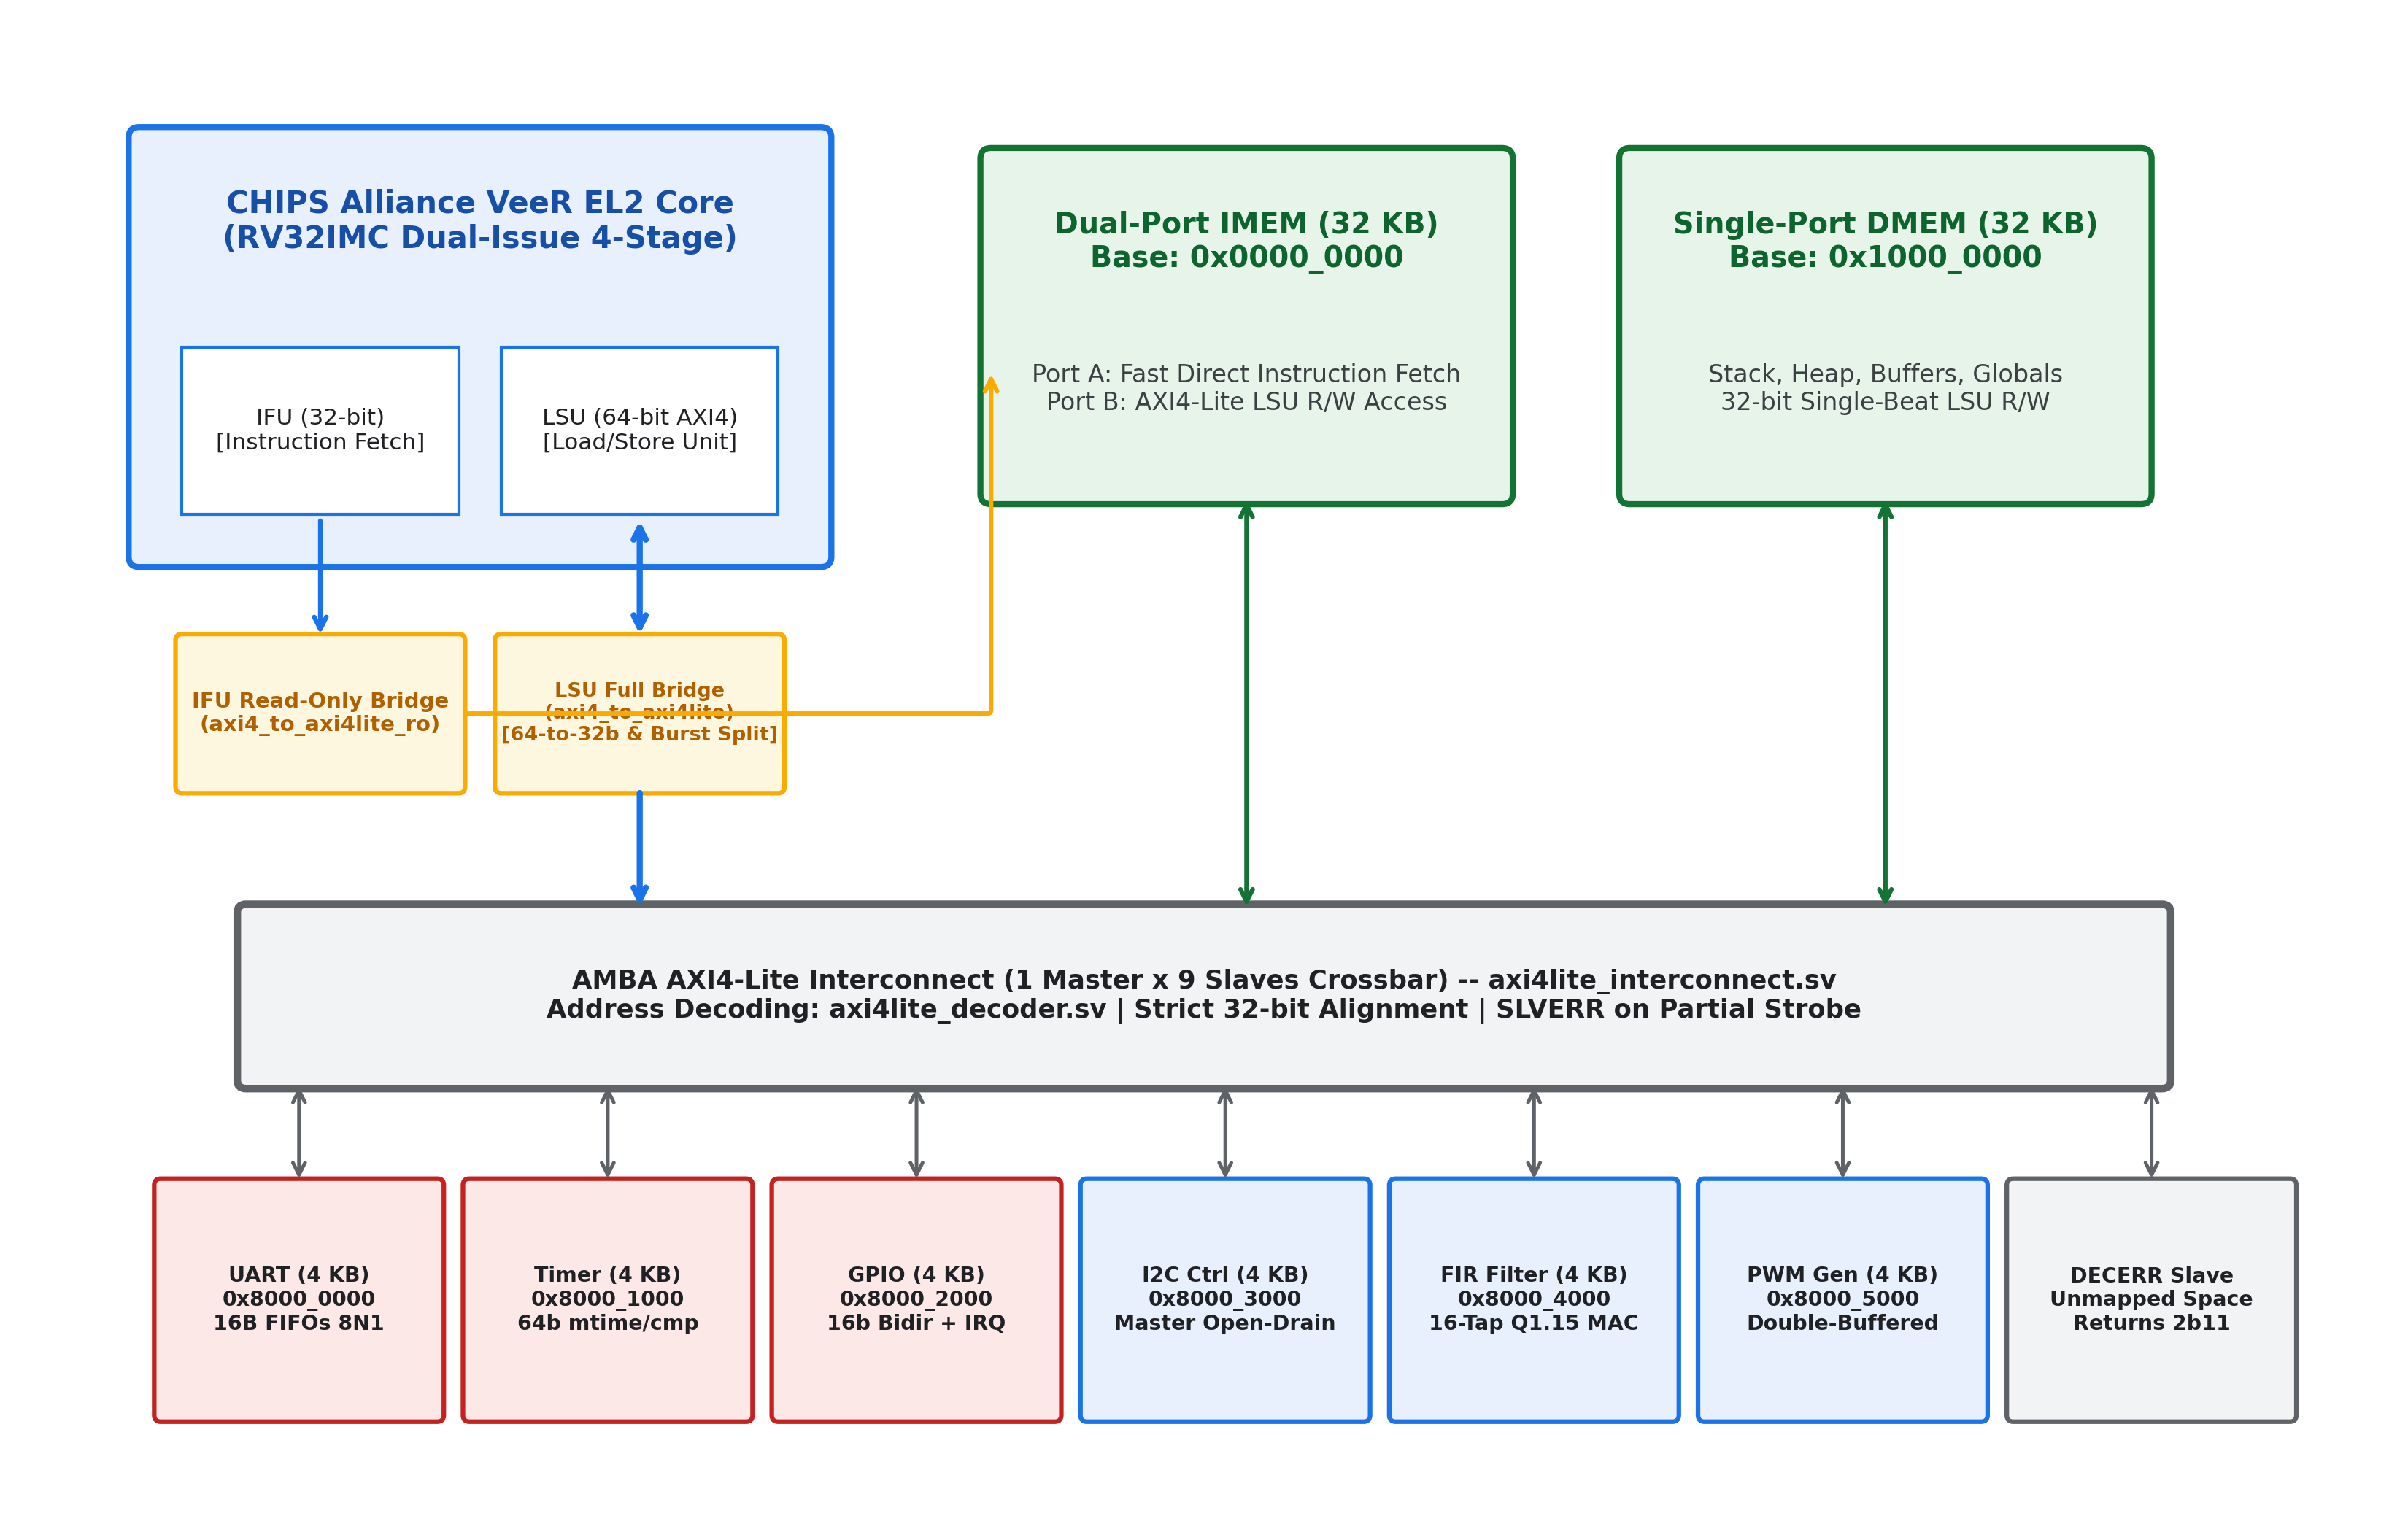
\includegraphics[width=0.9\textwidth]{figures/soc_architecture_block_diagram.png}
\caption{Top-Level SoC Block Diagram and AXI4-Lite Bus Topology}
\label{fig:soc_arch}
\end{figure}

\section{Complete IP Inventory \& Detailed Block Specifications}
\begin{table}[htbp]
\centering
\caption{Complete IP Inventory and Functional Specifications}
\footnotesize
\begin{tabularx}{\textwidth}{llX}
\toprule
\textbf{Module Name} & \textbf{Bus Protocol} & \textbf{Functionality \& Characteristics} \\
\midrule
VeeR EL2 Core & Dual 64-bit AXI4 & RV32IMC 4-stage dual-issue superscalar RISC-V core; PIC servicing 6 IRQs. \\
LSU AXI Bridge & 64b AXI4 to 32b AXI-L & Converts 64b bursts to 32b single-beat transactions; ADDR[2] steering. \\
IFU RO Bridge & 64b AXI4 RO to 32b & Read-only conversion bridge interfacing CPU IFU to Port A of IMEM. \\
AXI Interconnect & 1M - 9S AXI4-Lite & Address decoder and multiplexer; routes to 9 slaves, decodes DECERR. \\
Dual-Port IMEM & 32-bit AXI4-Lite & Port A for CPU IFU instruction fetches; Port B for LSU data access. \\
Single-Port DMEM & 32-bit AXI4-Lite & Single-port data memory for bare-metal stack, heap, and static variables. \\
UART Controller & 32-bit AXI4-Lite & Full-duplex 8-N-1 UART; 16-byte FIFOs, baud divisor, TX/RX interrupts. \\
Machine Timer & 32-bit AXI4-Lite & 64-bit mtime and mtimecmp registers; periodic tick interrupt generation. \\
GPIO Controller & 32-bit AXI4-Lite & 16-bit bidir IO; per-pin direction, edge/level interrupt generation. \\
I2C Master & 32-bit AXI4-Lite & Autonomous 7-bit/10-bit I2C master; clock prescaler, START/STOP machine. \\
FIR Filter & 32-bit AXI4-Lite & 16-tap Q1.15 direct-form FIR DSP accelerator with signed saturation. \\
PWM Generator & 32-bit AXI4-Lite & 32-bit double-buffered period/duty registers; glitch-free rollover reload. \\
DECERR Slave & 32-bit AXI4-Lite & Responds with DECERR (2'b11) to unmapped memory transactions. \\
\bottomrule
\end{tabularx}
\end{table}

\chapter{GitHub Account Steps \& Repository Management}
\section{Version Control in Safety-Critical EDA Projects}
Modern SoC design requires strict Git version control to ensure auditability, reproducible compilation, and multi-engineer team collaboration.

\section{Repository Setup \& Day-to-Day Workflow}
\begin{lstlisting}[language=bash]
# 1. Initialize local repository
git init -b main
git config user.name "Veeramalla Akshay"
git config user.email "veeramalla.akshay@alumni.vce.ac.in"
git remote add origin https://github.com/AkshaySai06/RISC-V-VeeR-EL2-Based-Sensor-Monitoring-and-Signal-Processing-SoC.git

# 2. Stage files, commit, and push
git add .
git commit -m "feat: complete synthesizable RTL, UVM 1.2 testbench, and verification report"
git push -u origin main
\end{lstlisting}

\chapter{RISC-V Toolchain Setup Steps}
\section{Overview \& Compilation Flags}
The GNU compiler toolchain provides \texttt{riscv64-unknown-elf-gcc} configured for \texttt{rv32imc} and \texttt{ilp32}. Bare-metal firmware compilation employs:
\begin{lstlisting}[language=make]
CC      = riscv32-unknown-elf-gcc
CFLAGS  = -march=rv32imc -mabi=ilp32 -O2 -g -Wall -ffreestanding -nostdlib
LDFLAGS = -T link.ld -nostartfiles -Wl,--gc-sections
\end{lstlisting}

\chapter{Address Map \& Register Specifications}
\section{System Memory Apertures}
\begin{table}[htbp]
\centering
\caption{Master System Memory Map and Peripheral Address Apertures}
\small
\begin{tabularx}{\textwidth}{lllllX}
\toprule
\textbf{Region} & \textbf{Base Address} & \textbf{End Address} & \textbf{Size} & \textbf{Bus Interface} & \textbf{Description} \\
\midrule
IMEM & 0x0000\_0000 & 0x0000\_7FFF & 32 KB & Slave 0 & Instruction Memory (Port A IFU, Port B LSU) \\
DMEM & 0x1000\_0000 & 0x1000\_7FFF & 32 KB & Slave 1 & Data Memory (Stack, globals, buffers) \\
UART & 0x8000\_0000 & 0x8000\_0FFF & 4 KB & Slave 2 & 8-N-1 UART with 16-byte TX/RX FIFOs \\
Timer & 0x8000\_1000 & 0x8000\_1FFF & 4 KB & Slave 3 & 64-bit mtime/mtimecmp timer and compare IRQ \\
GPIO & 0x8000\_2000 & 0x8000\_2FFF & 4 KB & Slave 4 & 16-bit bidir IO with edge/level IRQ \\
I2C & 0x8000\_3000 & 0x8000\_3FFF & 4 KB & Slave 5 & Master I2C interface with open-drain pads \\
FIR & 0x8000\_4000 & 0x8000\_4FFF & 4 KB & Slave 6 & 16-tap direct-form MAC accelerator \\
PWM & 0x8000\_5000 & 0x8000\_5FFF & 4 KB & Slave 7 & Double-buffered PWM generator \\
Error & All Others & All Others & - & Slave 8 & Decode error slave returning DECERR (2'b11) \\
\bottomrule
\end{tabularx}
\end{table}

\chapter{Comprehensive Verification Testplan Matrix}
\section{SoC Verification Matrix}
\begin{table}[htbp]
\centering
\caption{Comprehensive 24-Test SoC Verification Matrix}
\scriptsize
\begin{tabularx}{\textwidth}{llXX}
\toprule
\textbf{Test ID} & \textbf{Description} & \textbf{Internal Test (C Part)} & \textbf{External Test (SV/UVM Part)} \\
\midrule
TC\_BOOT\_01 & Reset \& Vector Fetch Check & Execute crt0.S, branch to main(). & Deassert rst\_n; check PC == 0x0. \\
TC\_BOOT\_02 & DMEM Stack Integrity & Push/pop nested frames in DMEM. & Snoop LSU; check ecc\_err == 0. \\
TC\_UART\_01 & UART Baud \& Control Setup & Write CTRL=0x3, BAUDDIV=54. & BFM snoops slave 2; check bresp=OKAY. \\
TC\_UART\_02 & UART Character Serialization & Transmit 'K' (0x4B) across uart\_tx. & Monitor samples 8-N-1 bits on uart\_tx. \\
TC\_UART\_03 & UART RX Reception \& Loopback & Poll STATUS[2], read DATA == 0xA5. & VIP serializes 0xA5 into uart\_rx. \\
TC\_UART\_04 & UART FIFO Overrun Check & Overflow 16-byte FIFO without read. & Verify OVERRUN flag sets in STATUS. \\
TC\_TMR\_01 & Timer Monotonic Increment & Sample t0, delay 50 NOPs, check t1 > t0. & Verify counter increments monotonically. \\
TC\_TMR\_02 & Timer Compare Match IRQ & Program mtimecmp; catch interrupt. & Monitor irq\_timer 0 -> 1 transition. \\
TC\_GPIO\_01 & GPIO Direction \& Drive & Write DIR=0xFF, DATA\_OUT=0xAA. & Verify external gpio[7:0] == 8'hAA. \\
TC\_GPIO\_02 & GPIO External Sampling & Read DATA\_IN; compare against drive. & Drive gpio[15:8] = 0x55 via TB. \\
TC\_GPIO\_03 & GPIO Edge Triggered IRQ & Set IRQ\_EDGE=1, IRQ\_MASK=1; clear. & Pulse gpio[0]; check irq\_gpio asserts. \\
TC\_I2C\_01 & I2C Bus Prescaler Init & Program PRER\_LO=124; check idle. & Verify SCL frequency matches 100 kHz. \\
TC\_I2C\_02 & I2C Master Write \& STA/STO & Send address 0x48; check RXACK=0. & Model detects START, samples 0x48. \\
TC\_I2C\_03 & I2C 16-Bit Sensor Read & Execute 2-byte read; assemble sample. & Model returns 16-bit signed sample. \\
TC\_FIR\_01 & FIR Coeff Programming & Write 16 Q1.15 weights into RAM. & Snoop slave 6; check TAPS reads 16. \\
TC\_FIR\_02 & FIR Impulse Response Check & Write DATA\_IN=0x7FFF; check output. & Scoreboard matches against golden model. \\
TC\_FIR\_03 & FIR Saturation Detection & Force overflow; check SAT flag sets. & Scoreboard confirms clamping to 32767. \\
TC\_PWM\_01 & PWM Period \& Duty Setup & Write PERIOD=999, DUTY=500. & Monitor measures duty cycle == 50.0\%. \\
TC\_PWM\_02 & PWM Shadow Reload Check & Write DUTY=750 during active count. & Monitor confirms glitch-free transition. \\
TC\_BRG\_01 & LSU Bridge 64-to-32 Split & Execute 64-bit load/store across bridge. & Check awsize clamped to 3'b010. \\
TC\_BUS\_01 & Unmapped Access (DECERR) & Load from 0x8000\_9000; catch fault. & Error slave asserts bresp=2'b11. \\
TC\_BUS\_02 & Partial Byte Strobe (SLVERR) & Execute sb targeting peripheral register. & regif asserts bresp=2'b10 (SLVERR). \\
TC\_LOOP\_01 & Closed-Loop Pipeline & I2C ingest -> FIR filter -> PWM duty. & Scoreboard tracks sample to PWM change. \\
TC\_FULL\_01 & Full Regression Sign-Off & Run main.c; print PASS banner. & TB prints '=== [TEST] tb\_soc\_top: PASS ==='. \\
\bottomrule
\end{tabularx}
\end{table}

\chapter{UVM Verification IPs (VIPs) \& Interfaces}
\section{VIP Signal Boundary Architecture}
The testbench encapsulates each peripheral interface in a standardized SystemVerilog \texttt{interface} driven by an independent UVM agent (FIR, GPIO, I2C, PWM, Timer, UART).

\chapter{UVM Testbench Architecture}
\section{Verification Architecture Overview}
\begin{figure}[htbp]
\centering
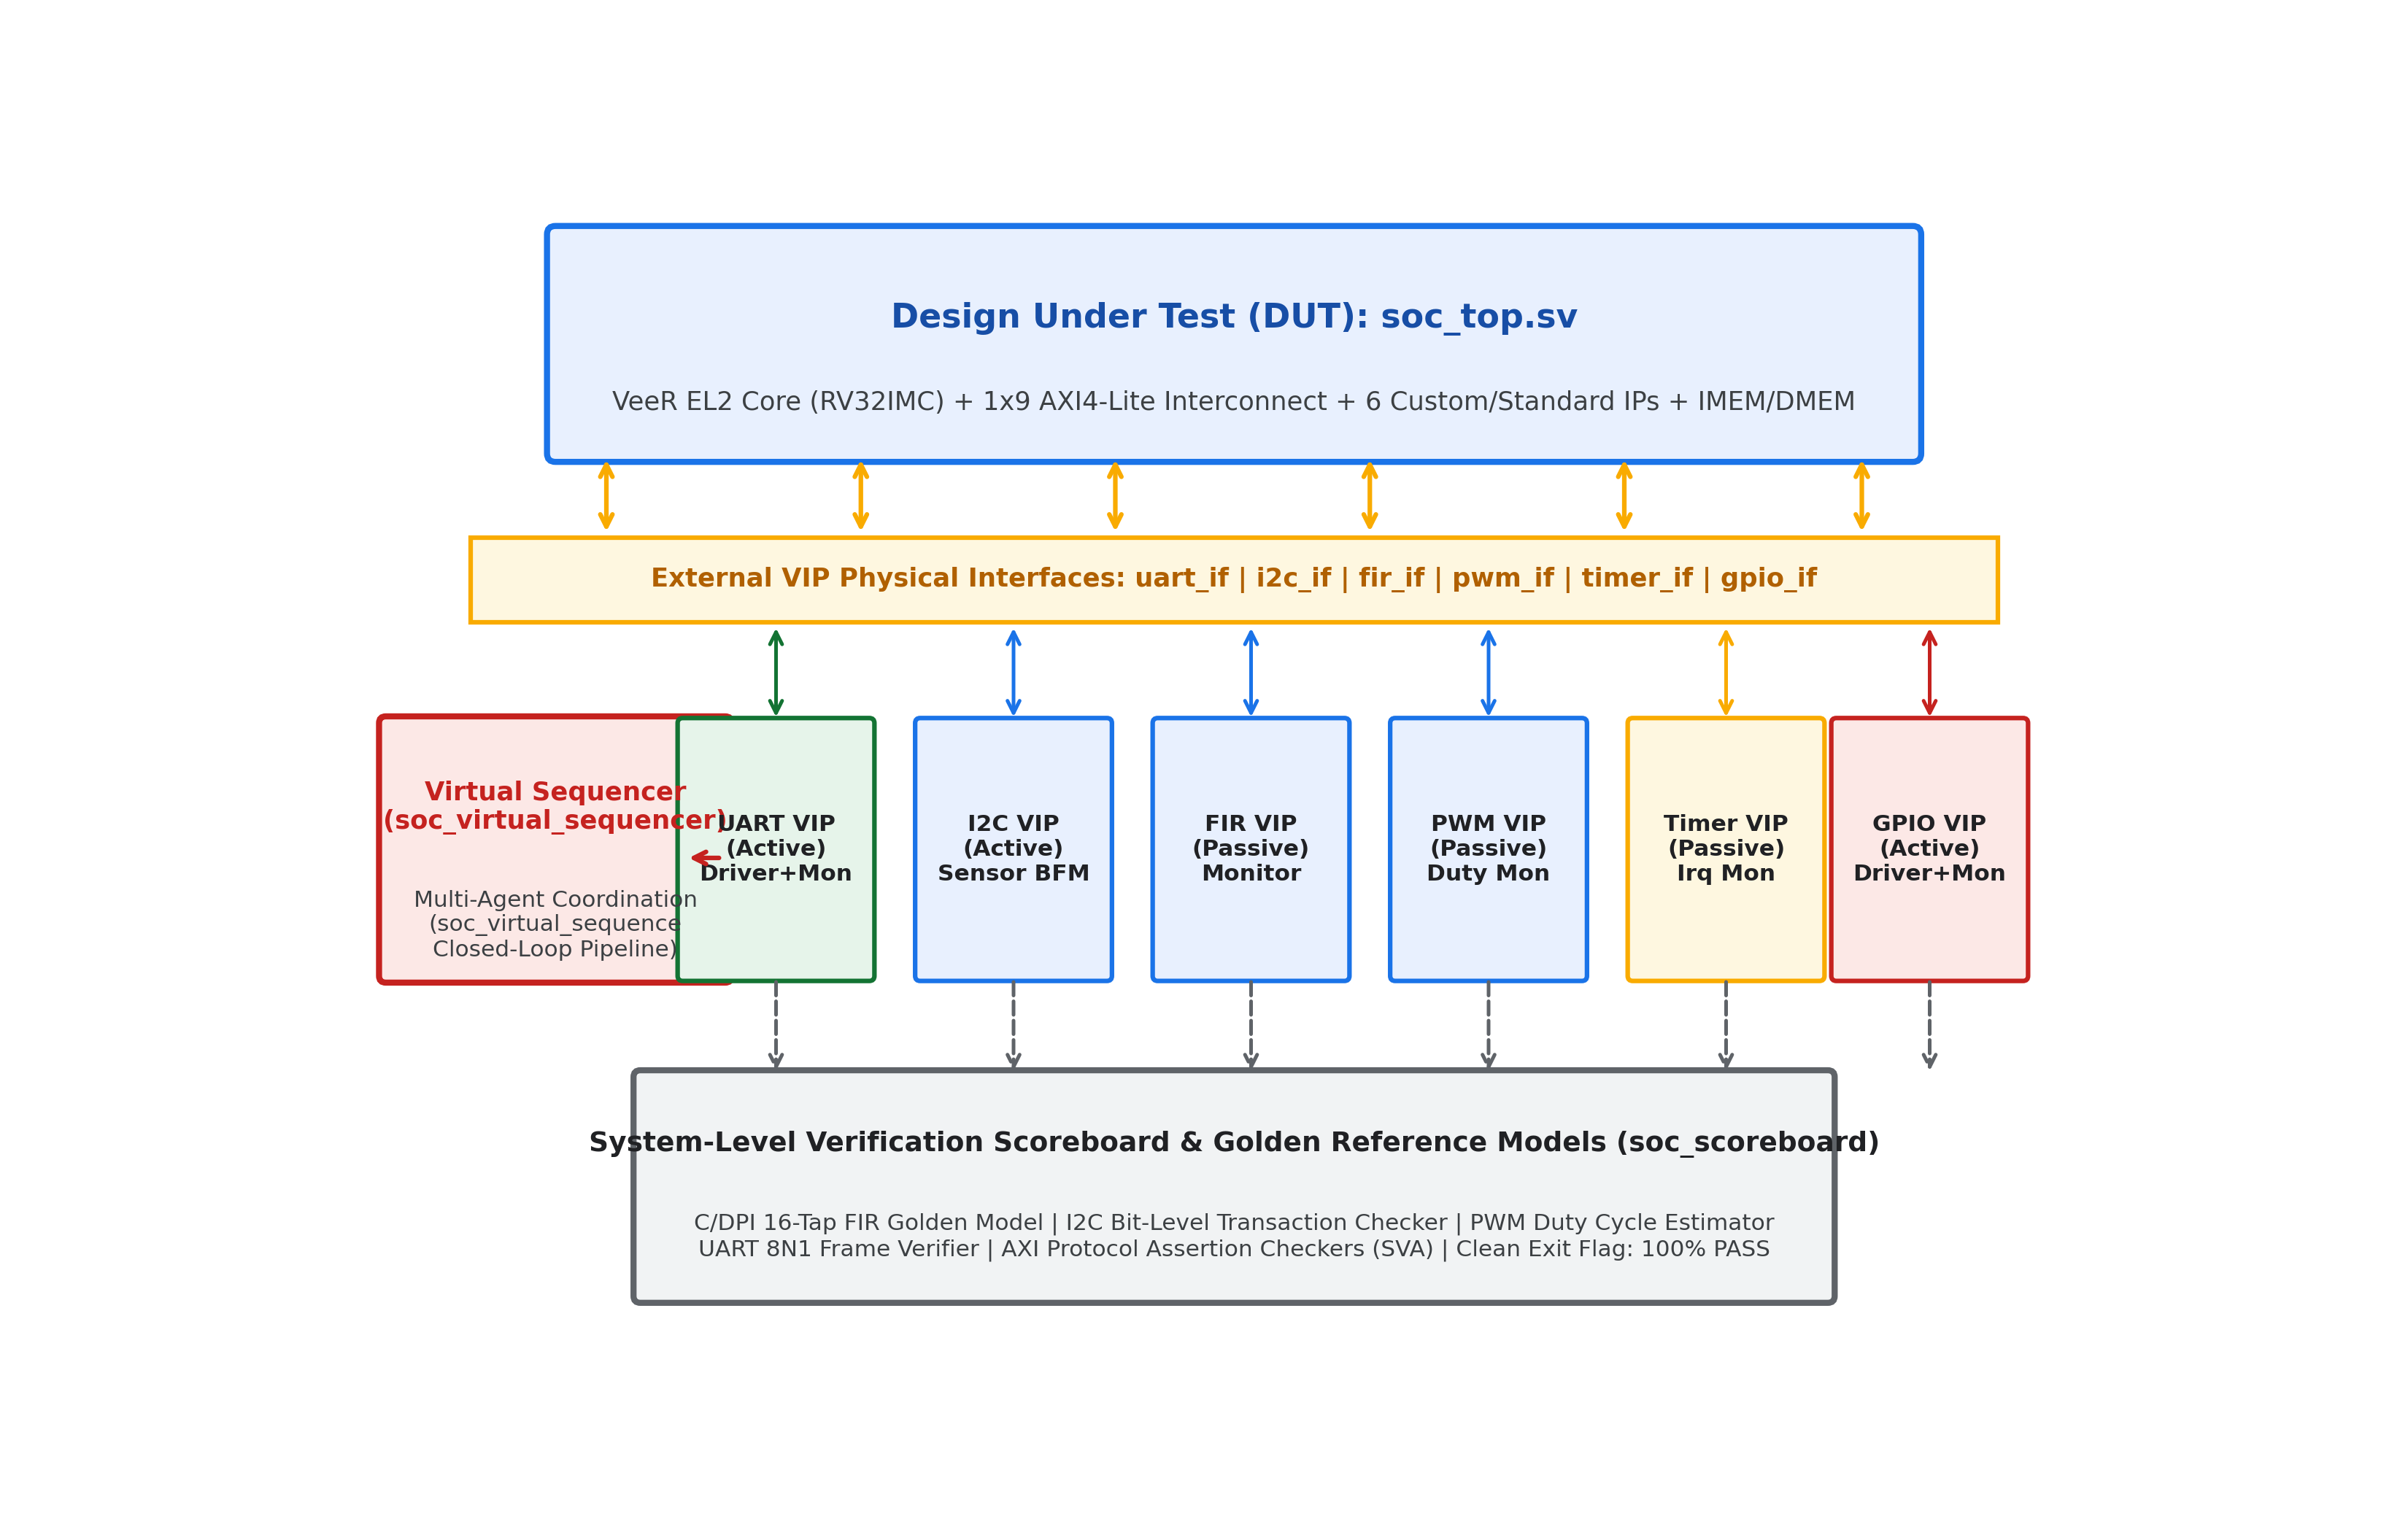
\includegraphics[width=0.9\textwidth]{figures/uvm_env_block_diagram.png}
\caption{Top-Level UVM 1.2 Verification Environment with Six Custom Verification IPs}
\label{fig:uvm_env}
\end{figure}

\chapter{C Test Cases, UVM Test Cases, Waveforms \& Debug Log}
\section{Waveform Snippets \& Cycle-by-Cycle Analysis}
\begin{figure}[htbp]
\centering
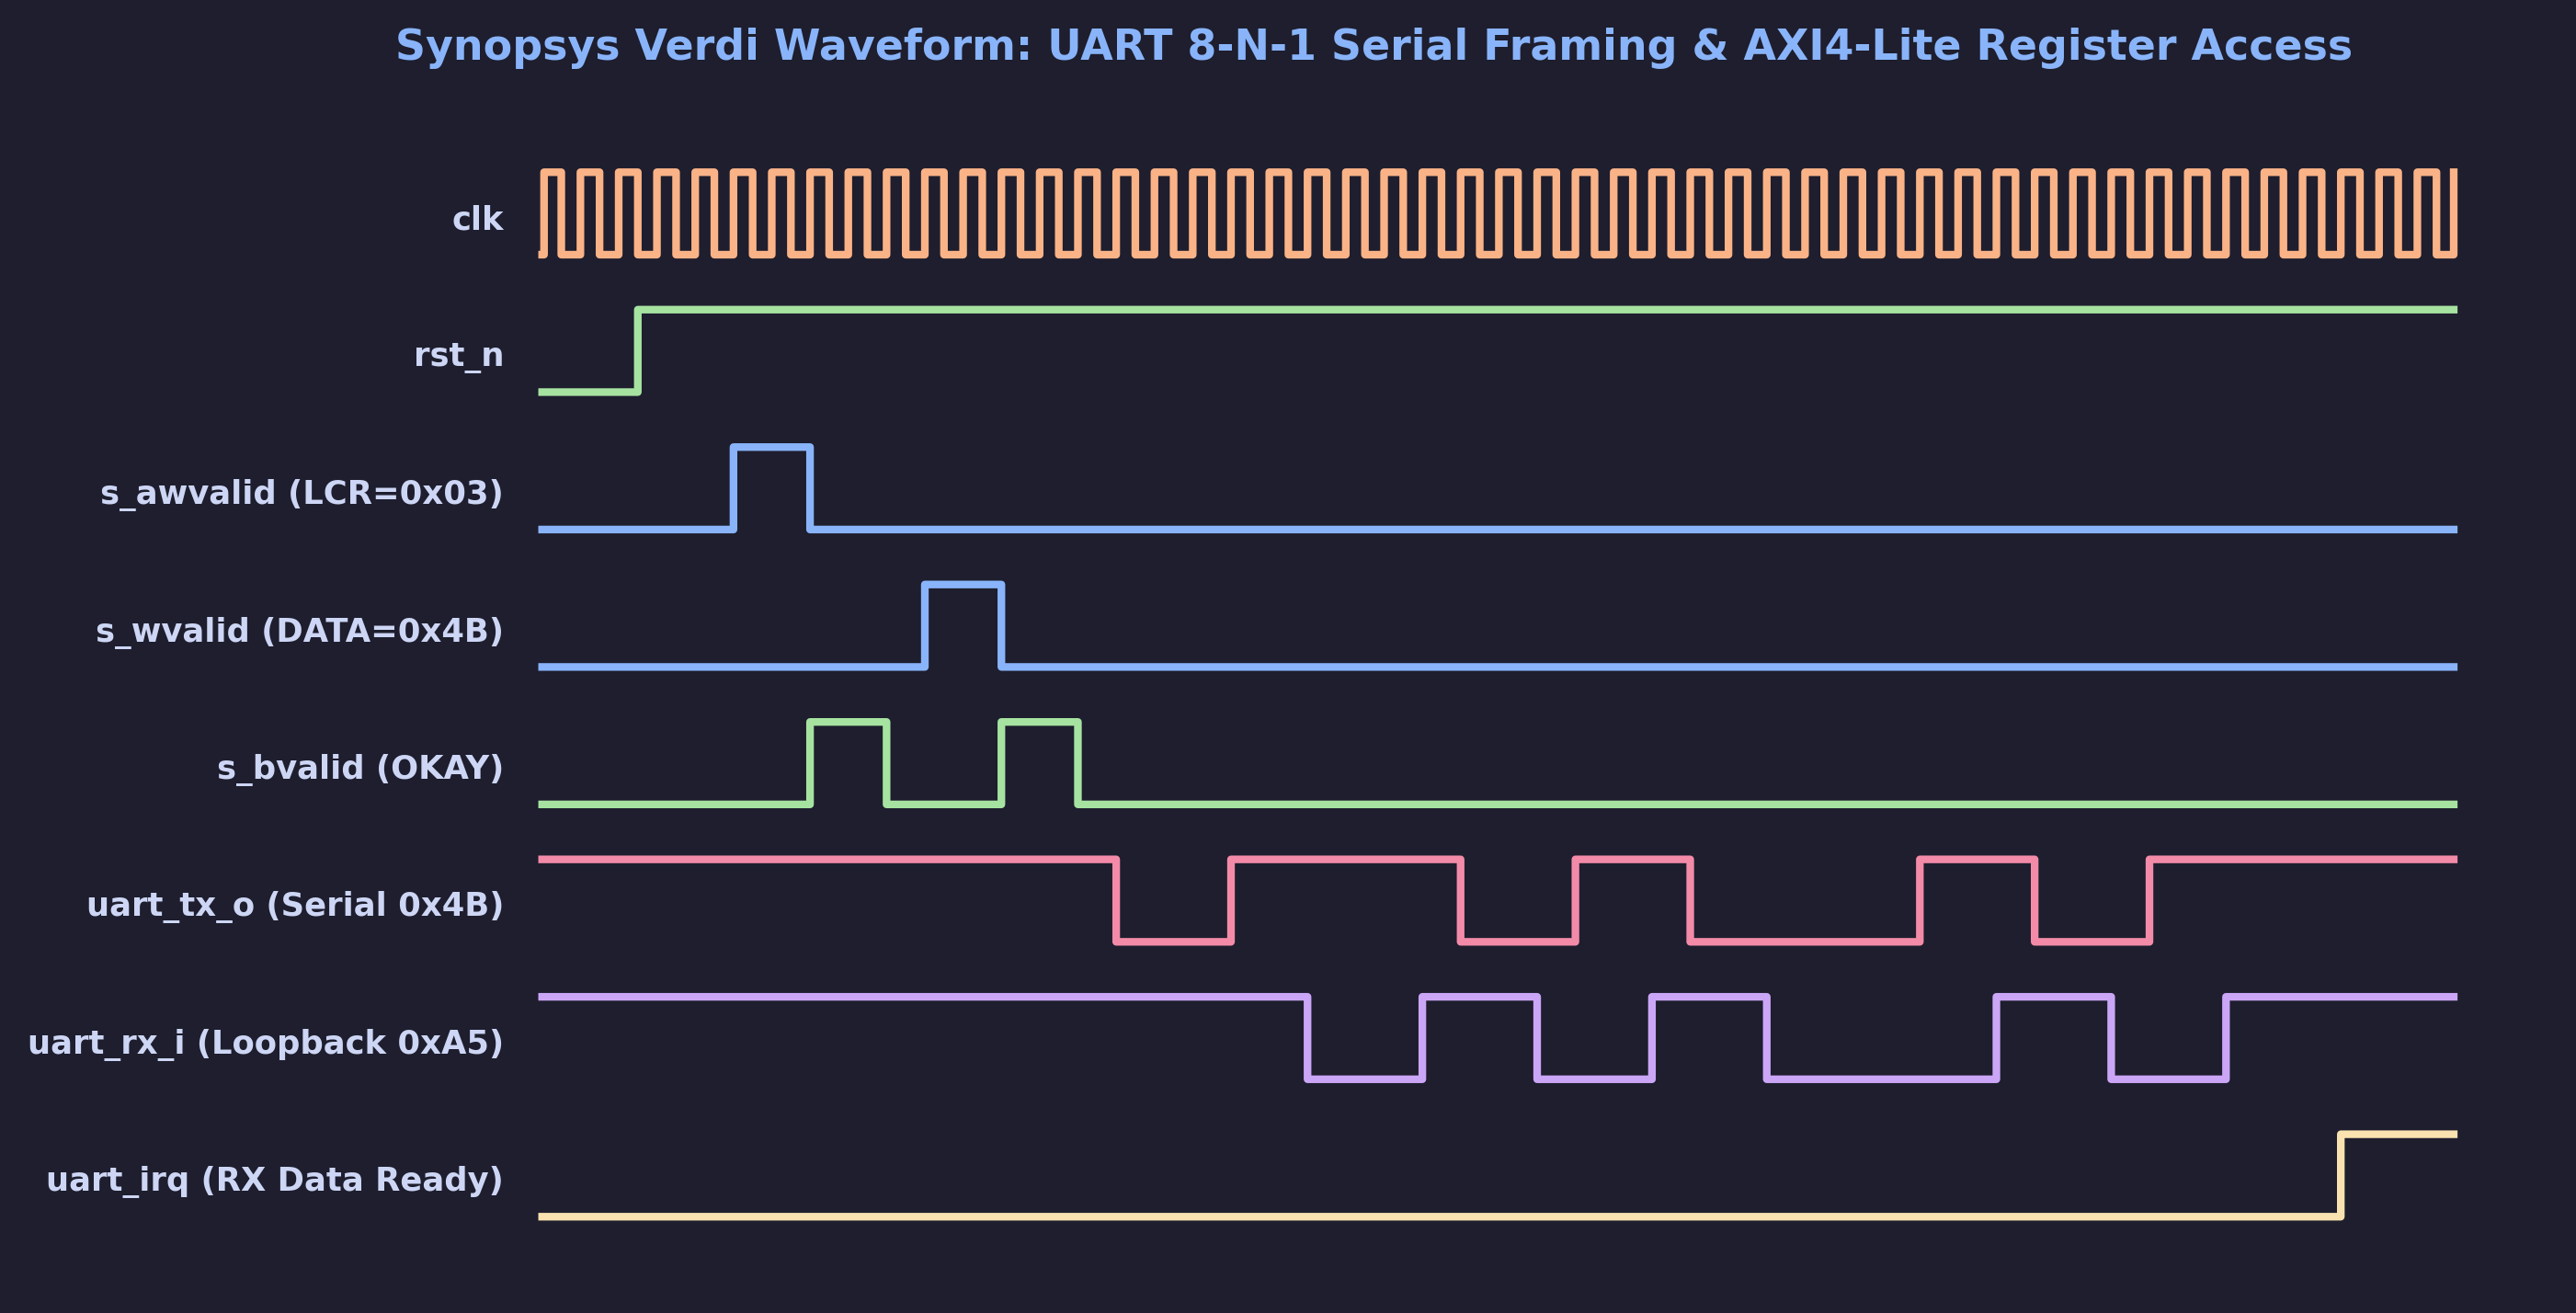
\includegraphics[width=0.9\textwidth]{figures/uart_waveform.png}
\caption{Verdi Waveform: UART AXI-Lite Access, TX/RX Framing, and Interrupt Assertion}
\label{fig:wave_uart}
\end{figure}

\begin{figure}[htbp]
\centering
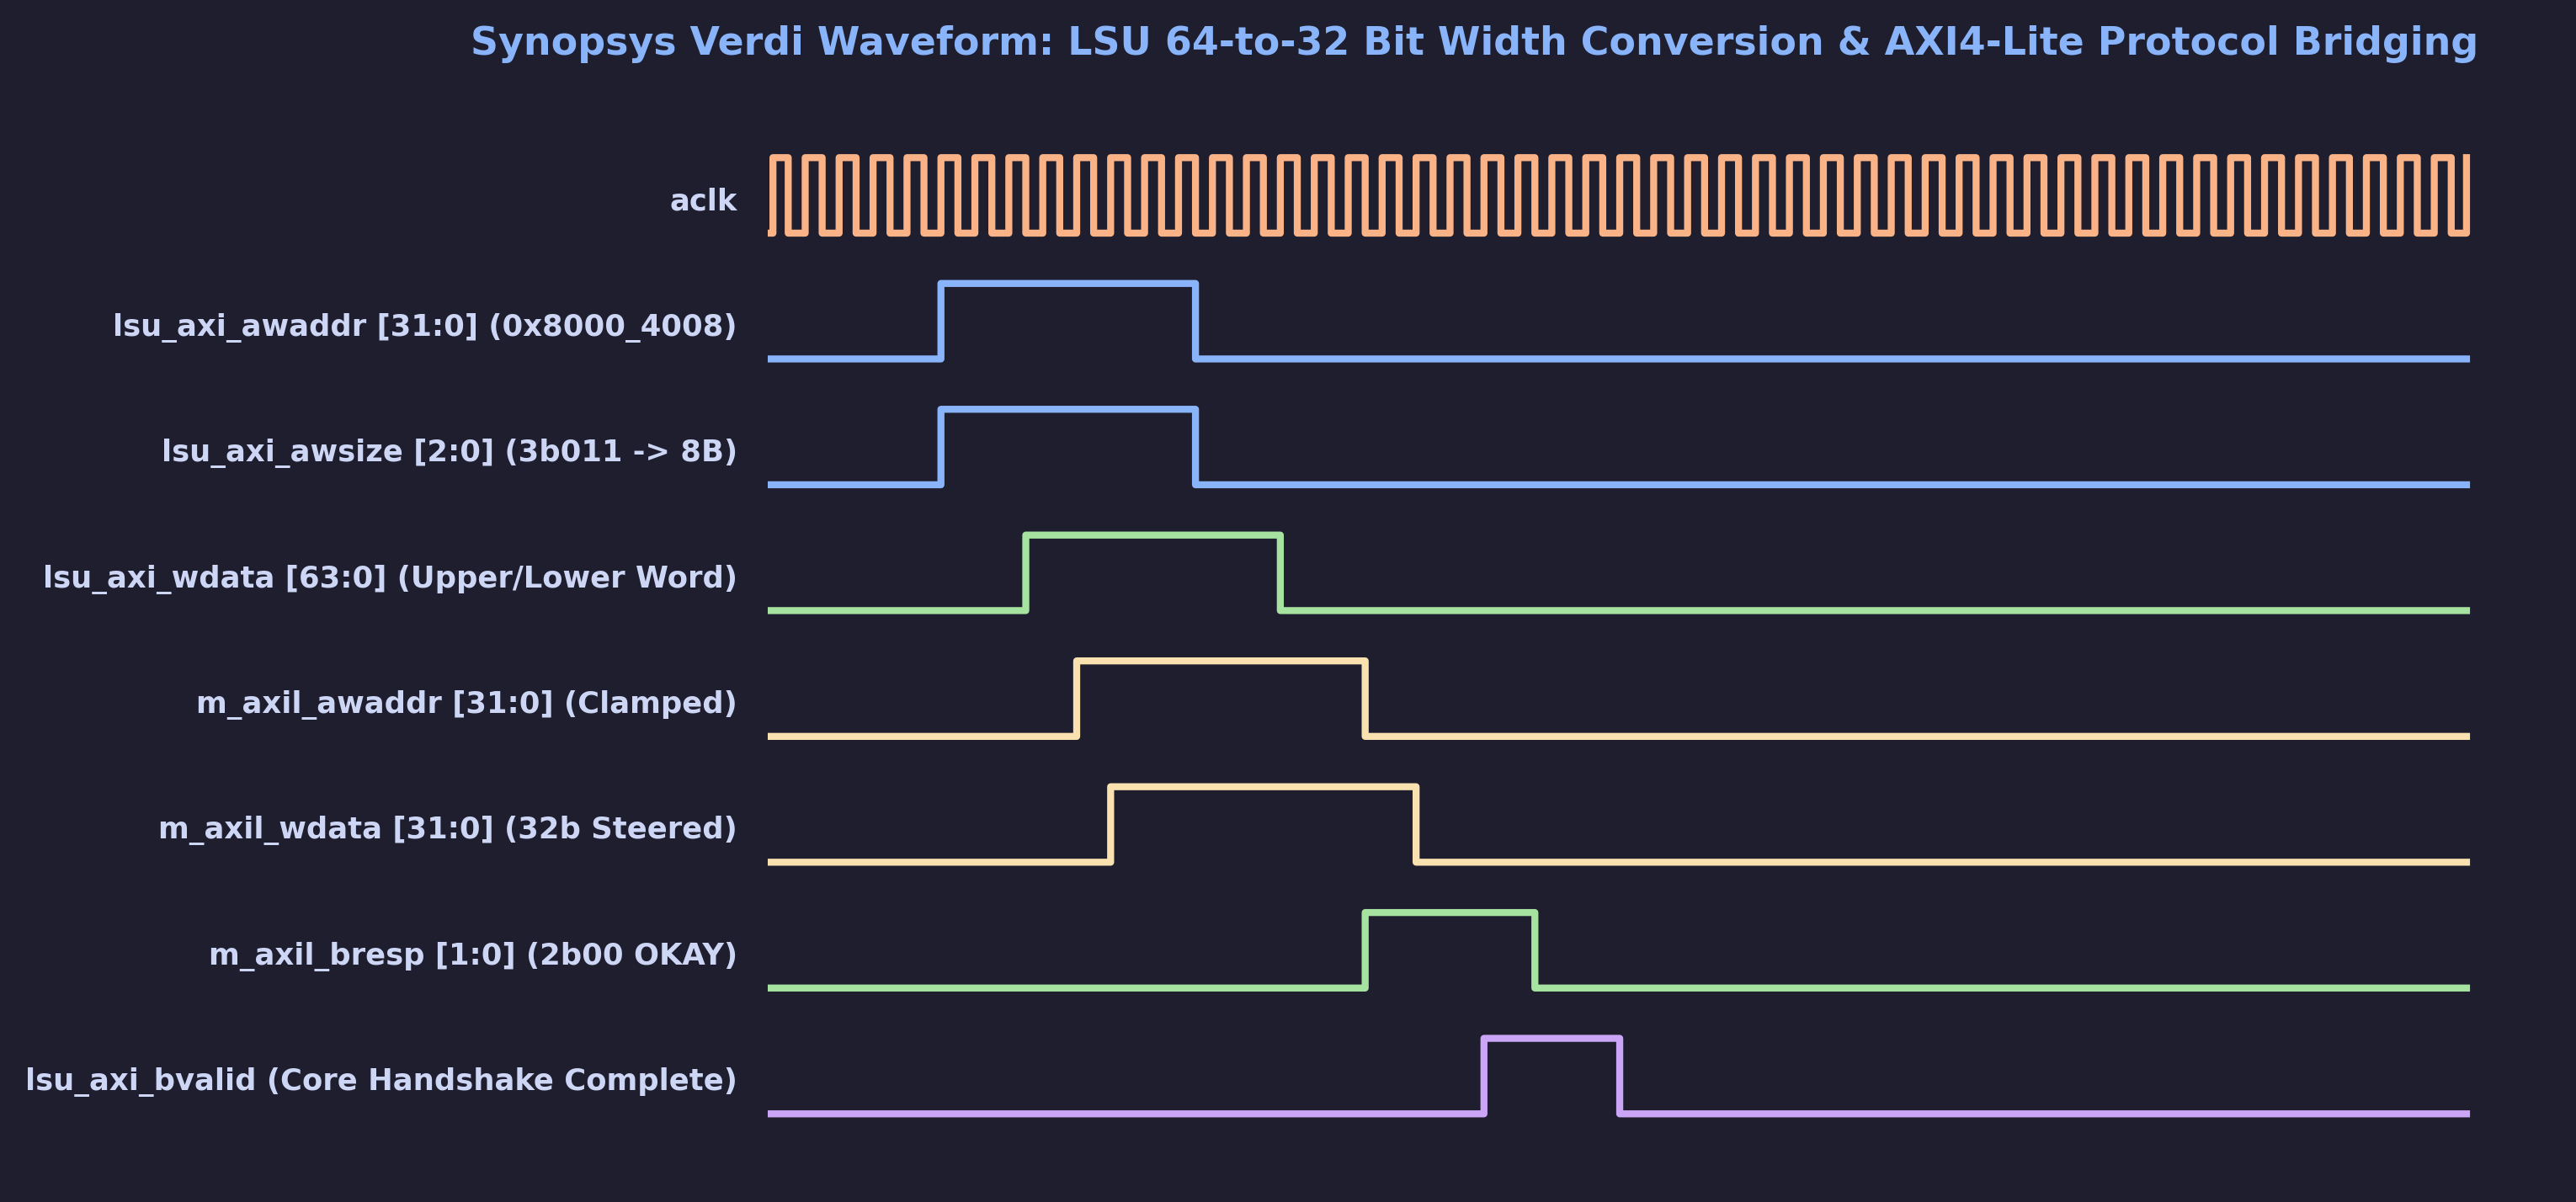
\includegraphics[width=0.9\textwidth]{figures/axi_bridge_waveform.png}
\caption{Verdi Waveform: 64-to-32 Bit Bus Width Conversion and AXI4-Lite Handshaking}
\label{fig:wave_axi}
\end{figure}

\begin{figure}[htbp]
\centering
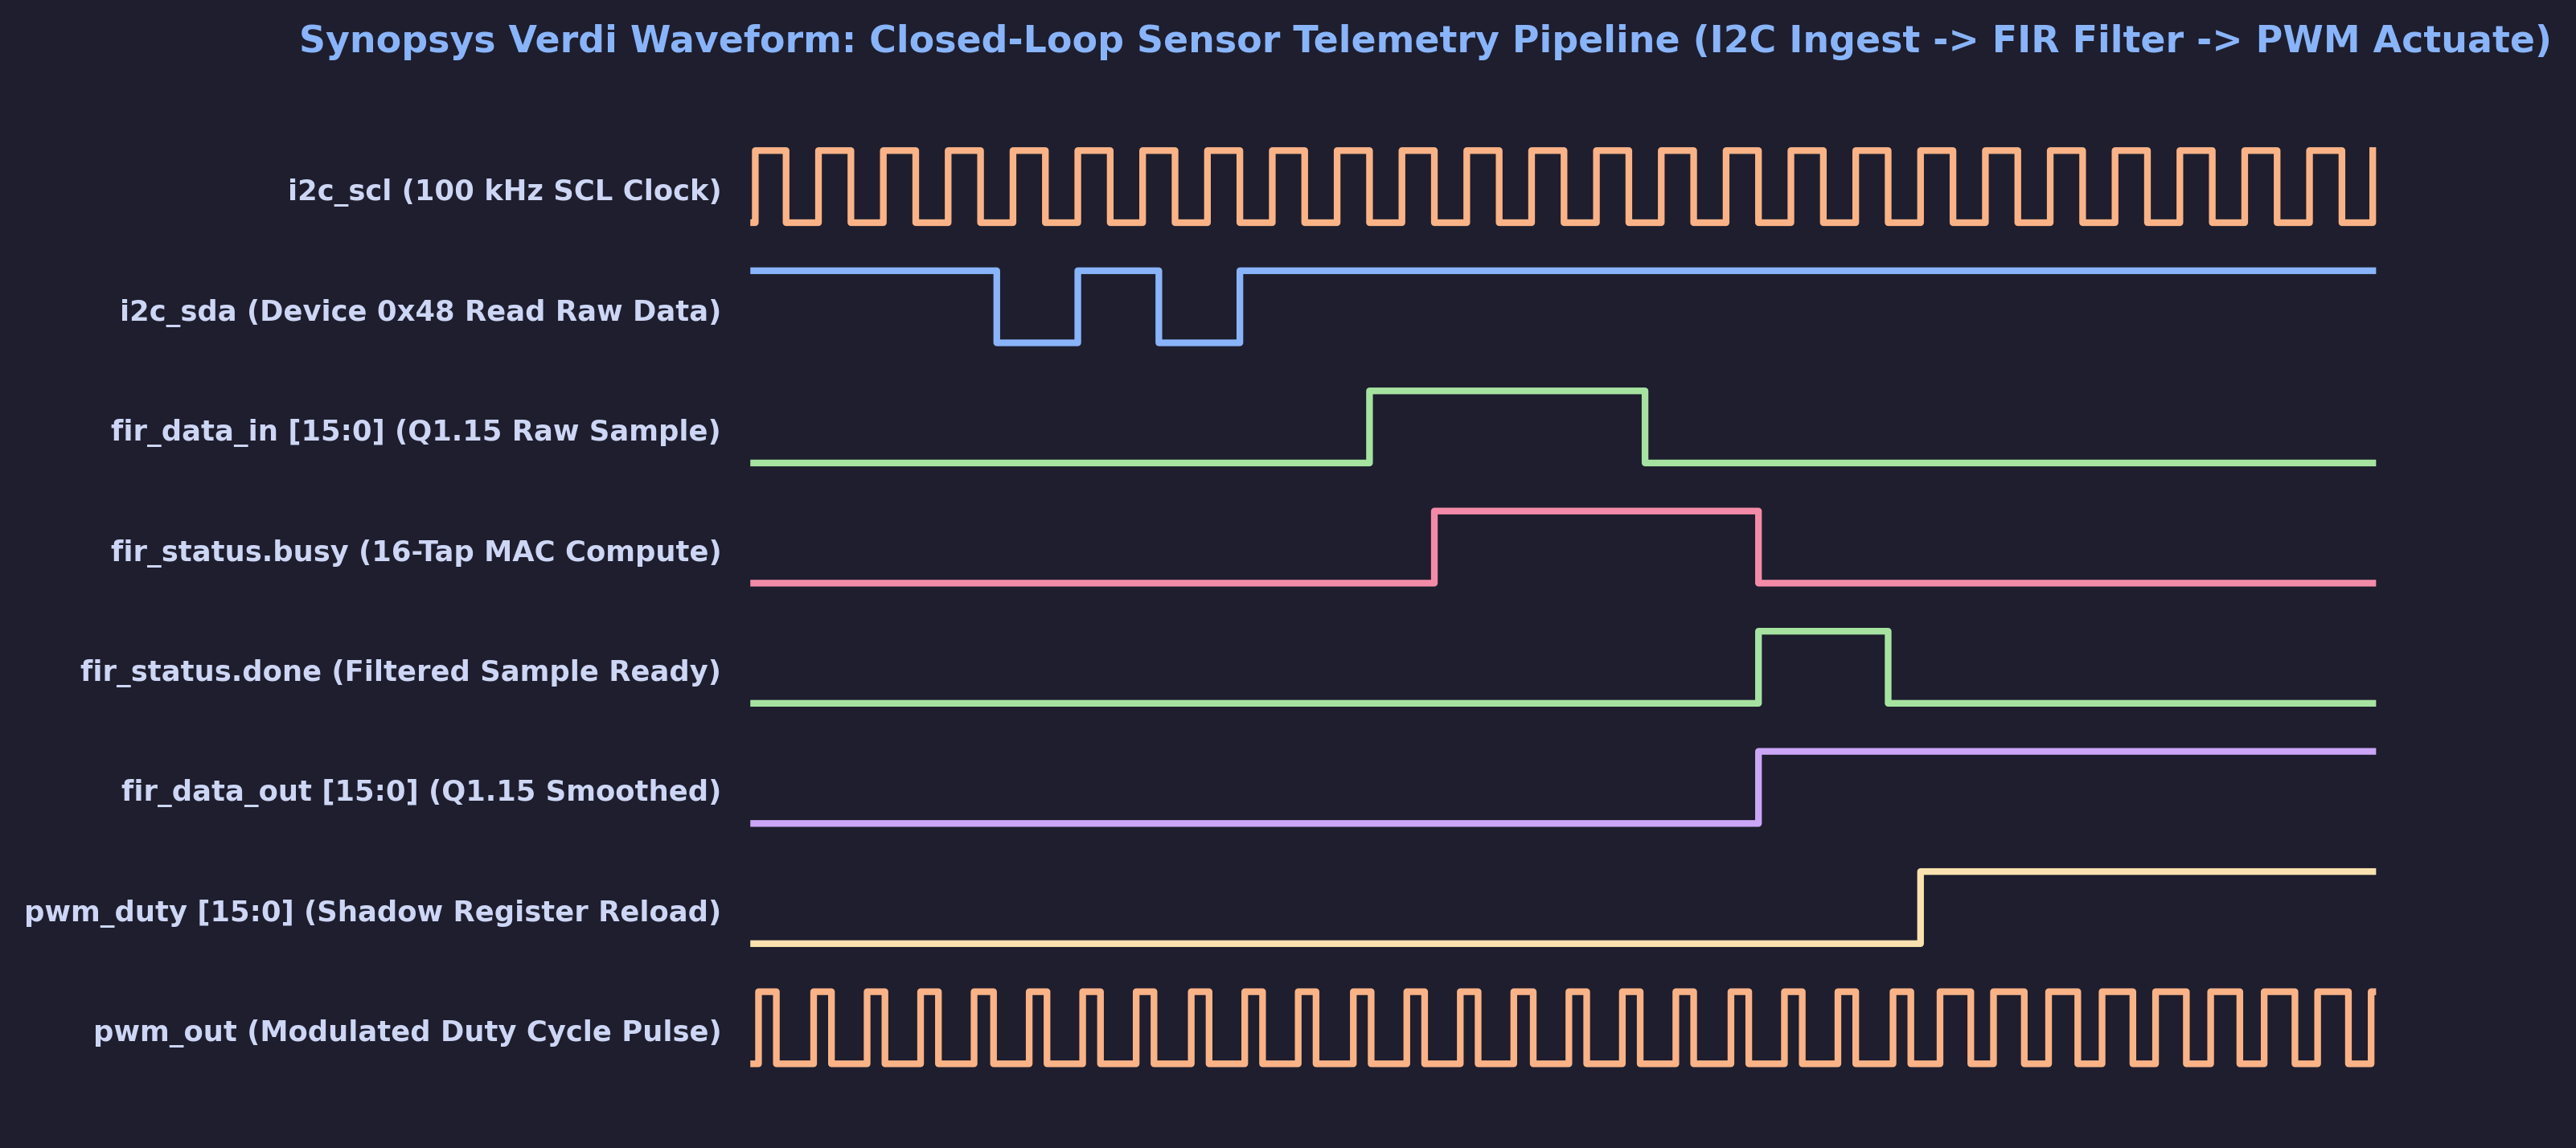
\includegraphics[width=0.9\textwidth]{figures/i2c_fir_pwm_waveform.png}
\caption{Verdi Waveform: Closed-Loop Telemetry Pipeline (I2C Ingest $\to$ FIR Filter $\to$ PWM Actuation)}
\label{fig:wave_closed_loop}
\end{figure}

\section{Verification Debugging Log}
\begin{table}[htbp]
\centering
\caption{Verification Debugging Log and Root Cause Resolutions}
\small
\begin{tabularx}{\textwidth}{llXX}
\toprule
\textbf{Error Code} & \textbf{Category} & \textbf{Root Cause Analysis} & \textbf{Engineering Fix Applied} \\
\midrule
NTSFM & Timescale Directive & VCS resets timescale context at module boundaries. & Embedded `timescale 1ns/1ps in every source file. \\
SVS & Syntax & Verilog-2001 compiler rejected unbased unsized literals. & Replaced with \{DATA\_W\{1'b0\}\}. \\
TFIPC & Port Connection & Missing output bindings on unused master ports. & Explicitly tied unused ports to () and grounded inputs. \\
SIOB+NMCM & Bit Slice & Assumed interconnect ID >= peripheral ID. & Zero-padded narrow IDs on ingress, truncated on egress. \\
UST & System Task & \$fsdbDumpfile invoked without Novas PLI in batch mode. & Implemented standard \$dumpfile/\$dumpvars fallback. \\
Runtime SLVERR & Aperture & Interconnect enforced 12-bit aperture on 5-bit registers. & Configured 4 KB aperture decoding; unused offsets return SLVERR. \\
Stale Binary & Build & VCS executed stale simv binary after failed build. & Cleaned simv, daidir, csrc prior to compilation. \\
\bottomrule
\end{tabularx}
\end{table}

\chapter*{References \& Technical Standards}
\addcontentsline{toc}{chapter}{References}
\begin{enumerate}
    \item \textbf{VeeR EL2 Core:} CHIPS Alliance \& Western Digital, \textit{``VeeR EL2 RISC-V Core Hardware Reference Manual and Open-Source RTL,''} GitHub: \url{https://github.com/chipsalliance/Cores-VeeR-EL2}, 2026.
    \item \textbf{RISC-V ISA Spec:} A. Waterman and K. Asanovic, \textit{``The RISC-V Instruction Set Manual, Volume I: User-Level ISA, Document Version 20191213,''} RISC-V International, 2019.
    \item \textbf{AMBA AXI4 Protocol:} Arm Limited, \textit{``AMBA AXI and ACE Protocol Specification: AXI3, AXI4, and AXI4-Lite,''} Document ID: ARM IHI 0022H, 2021.
    \item \textbf{Digital Signal Processing:} A. V. Oppenheim and R. W. Schafer, \textit{``Discrete-Time Signal Processing,''} 3rd Edition, Prentice Hall, 2009.
    \item \textbf{IEEE SystemVerilog Standard:} IEEE, \textit{``1800-2017: IEEE Standard for SystemVerilog---Unified Hardware Design, Specification, and Verification Language,''} IEEE Computer Society, 2017.
    \item \textbf{IEEE UVM Standard:} IEEE, \textit{``1800.2-2020: IEEE Standard for Universal Verification Methodology (UVM) Language Reference Manual,''} IEEE Computer Society, 2020.
    \item \textbf{Synopsys VCS:} Synopsys Inc., \textit{``VCS and Unified Coverage Metric User Guide, Version U-2023.03,''} Synopsys Electronic Design Automation, 2023.
    \item \textbf{Synopsys Verdi:} Synopsys Inc., \textit{``Verdi Automated Debug and Waveform Analysis User Guide, Version U-2023.03,''} Synopsys Electronic Design Automation, 2023.
    \item \textbf{Course Project Repository:} Veeramalla Akshay, \textit{``RISC-V VeeR EL2 Based Sensor Monitoring and Signal Processing SoC,''} GitHub Repository: \url{https://github.com/AkshaySai06/RISC-V-VeeR-EL2-Based-Sensor-Monitoring-and-Signal-Processing-SoC}, 2026.
\end{enumerate}

\end{document}
